%%%%%%%%%%%%%%%%%%%%%%%%%%%%%%%%%%%%%%%%%%%%%%%%%%%%%%%%%%%%%%%%%%%%%%%%%%%%%%
\documentclass[12pt,hidelinks]{article}

% 1. Load LaTeX packages
\usepackage{fontspec}
\usepackage{geometry}
\usepackage{lastpage}
\usepackage{fancyhdr}
\usepackage{hyperref}
\usepackage{amsmath}
\usepackage{amsthm}
\usepackage{xunicode}
\usepackage{listings}
\usepackage{color}
\usepackage{amssymb}

% 2. Define page dimensions and spacing
\geometry{top=1in, bottom=1in, left=1in, right=2in, marginparsep=4pt,
          marginparwidth=1in}
\setlength{\parindent}{0pt}
\setlength{\parskip}{12pt}

% 3. Set header, footer, and bibliography
\renewcommand{\headrulewidth}{0pt}
\pagestyle{fancyplain}
\fancyhf{}
\lfoot{}
\rfoot{page \thepage\ of \pageref{LastPage}}
\bibliographystyle{acm}

% 4. Set fonts for the document
\defaultfontfeatures{Mapping=tex-text}
\setromanfont{YaleNew}

% 5. Define custom code for book environments and commands
\DeclareMathOperator*{\argmin}{arg\,min}
\DeclareMathOperator*{\argmax}{arg\,max}
\newcommand{\code}[1]{\texttt{#1}}
\newcommand{\pkg}[1]{\textbf{#1}}

% 6. Define custom code for book environments and commands
\definecolor{verbgray}{gray}{0.9}
\definecolor{verbgray2}{gray}{0.975}

\lstnewenvironment{rcode}{%
  \lstset{backgroundcolor=\color{verbgray},
  frame=single,
  framerule=0pt,
  basicstyle=\ttfamily,
  keepspaces=true,
  columns=fullflexible}}{}

\lstnewenvironment{rres}{%
  \lstset{backgroundcolor=\color{verbgray2},
  frame=single,
  framerule=0pt,
  basicstyle=\ttfamily,
  keepspaces=true,
  columns=fullflexible}}{}

% 7. Define numbering scheme for equations (only needed for handout).
\numberwithin{equation}{section}
\setcounter{section}{1}

%%%%%%%%%%%%%%%%%%%%%%%%%%%%%%%%%%%%%%%%%%%%%%%%%%%%%%%%%%%%%%%%%%%%%%%%%%%%%%
\begin{document}

{\LARGE Lab Solutions 01}

\vspace*{12pt}

\textbf{1. Describe what the spaces $\Omega$ and $\mathcal{Y}$ would be for a
predictive modeling task that estimates whether an email message is either
spam or not spam.}

\vspace*{12pt}

The space $\Omega$ is all the possible values we would have for the number
of capital letters in the text, and is given by the positive integers:

\begin{align*}
\Omega &= \{ 0, 1, 2, 3, \ldots \} = \mathbb{Z}_{\geq 0}.
\end{align*}

The space $\mathcal{Y}$ are all of the possible values that are trying to
predict as outcomes of the spam detection. You could answer with either the
categories themselves:

\begin{align*}
\mathcal{Y} &= \{ \text{ham}, \text{spam} \}.
\end{align*}

Or their respective numeric codes as using my R example:


\begin{align*}
\mathcal{Y} &= \{ 0, 1 \}.
\end{align*}

Either is equally correct.

\vspace*{12pt}

\textbf{2. Describe what might be some possible columns of the dataset $X$ in
a task trying to predict the sale price for a used car.}

\vspace*{12pt}

The columns are the variables that we would use to predict the price of a
house. Possible answers include: (i) the square footage of the house, (ii)
the lot size, (iii) number of bedrooms, (iv) year build, (v) and the house's
zip code.

\vspace*{12pt}

\textbf{3. Assume that the feature matrix $X$ has only one column, with values
evenly distributed between $0$ and $1$, and the true function $f$ is
deterministic and defined such that to $y_i = x_i^2$. If our modeling
algorithm is only allowed to produce a $\widehat{f}$ equal to a linear
function of $x_i$, illustrate using a hand drawn plot how (in this case) the
low model complexity directly leads to model bias.}

\vspace*{12pt}

Rather than hand-draw, I will give you an example using an R plot:

% library(dplyr)
% library(ggplot2)

% df <- tibble(x = seq(0, 1, by = 0.05), y = x^2)
% beta <- coef(lm(y ~ x, data = df))
% df$yhat <- beta[1] + beta[2] * df$x

% ggplot(df, aes(x, y)) +
%   geom_point() +
%   geom_line(alpha = 0.5) +
%   geom_line(aes(y = yhat), alpha = 0.5, linetype="dashed") +
%   geom_segment(aes(xend = x, yend = yhat), data = filter(df, yhat > y),
%                color = "blue") +
%   geom_segment(aes(xend = x, yend = yhat), data = filter(df, yhat < y),
%                color = "red") +
%   theme_minimal()
% ggsave("figures/sol01-fig01.png", height=6, width=8)

\begin{center}
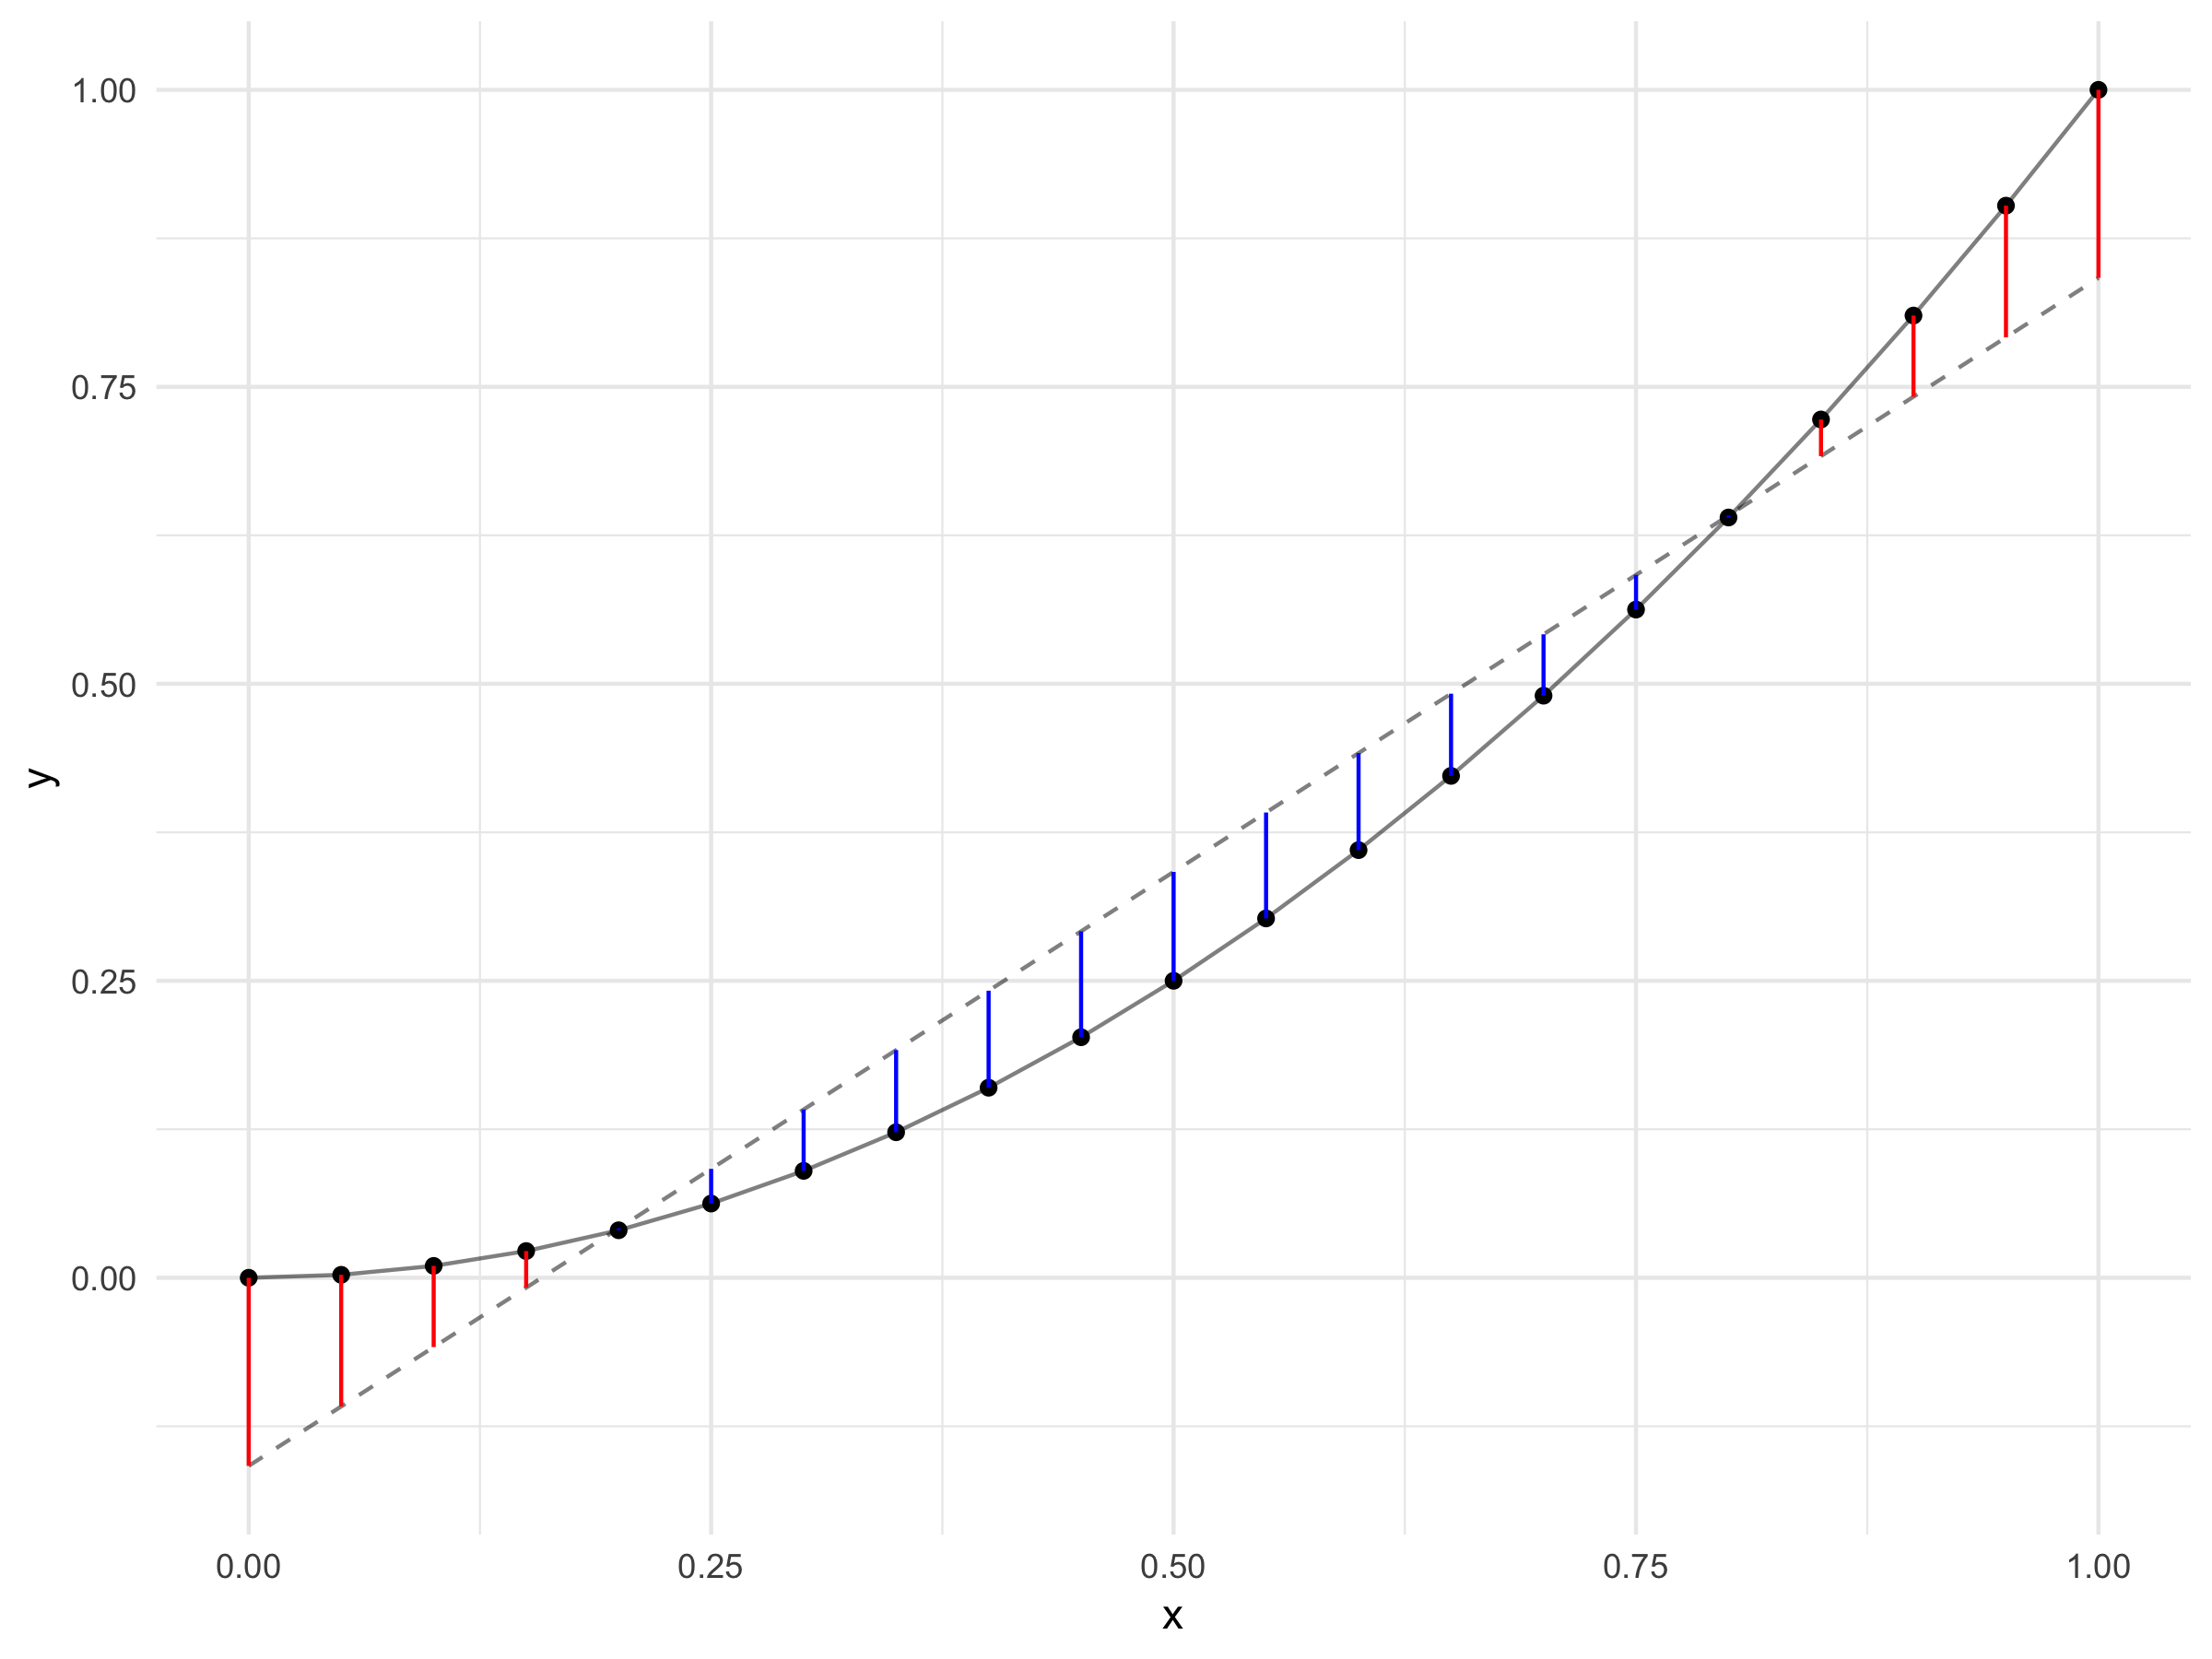
\includegraphics[width=\textwidth]{figures/sol01-fig01}
\end{center}

The `true' function $f(x)$ is given by the solid black line and our prediction
$\widehat{f}(x)$ is shown with the dashed line. The errors are given by the
colored vertical dashed bars. Points are consistently underpredicted where
the colors are red and overpredicted where the colors are blue. This shows
how the predicts are biased because the curve we fit is not complex enough to
capture the function $f(x)$.

\vspace*{12pt}

\textbf{4. Assume that the feature matrix $X$ has only one column, with values
evenly distributed between $0$ and $1$, and the true function $f$ is
deterministic and defined such that to $y_i = x_i^2$. If our modeling
algorithm is only allowed to produce a $\widehat{f}$ equal to a linear
function of $x_i$, illustrate using a hand drawn plot how (in this case) the
low model complexity directly leads to model bias.}

\vspace*{12pt}

I accidentally repeated this question. See answer above.

\vspace*{12pt}


\textbf{5. Using the same setup as in the previous question, but allowing
$\widehat{f}$ to take on any form, illustrate an example of a curve that has
been overfit to the data.}

\vspace*{12pt}

An overfit function $\widehat{f}$ is erroneously overly complex to fit the
observed data in a way that will not generalize to new data points.

% library(dplyr)
% library(ggplot2)

% df <- tibble(x = seq(0, 1, by = 0.05), y = x^2)
% df2 <- tibble(x = seq(0, 1, by = 0.001), y = x^2)
% df2$yhat <- df2$x^2 + sin(df2$x * (2 * pi * 20)) * df2$x * 2

% ggplot(df, aes(x, y)) +
%   geom_point() +
%   geom_line(alpha = 0.5) +
%   geom_line(aes(y = yhat), alpha = 0.5, linetype="dotted", data = df2) +
%   theme_minimal()
% ggsave("figures/sol01-fig02.png", height=6, width=8)

\begin{center}
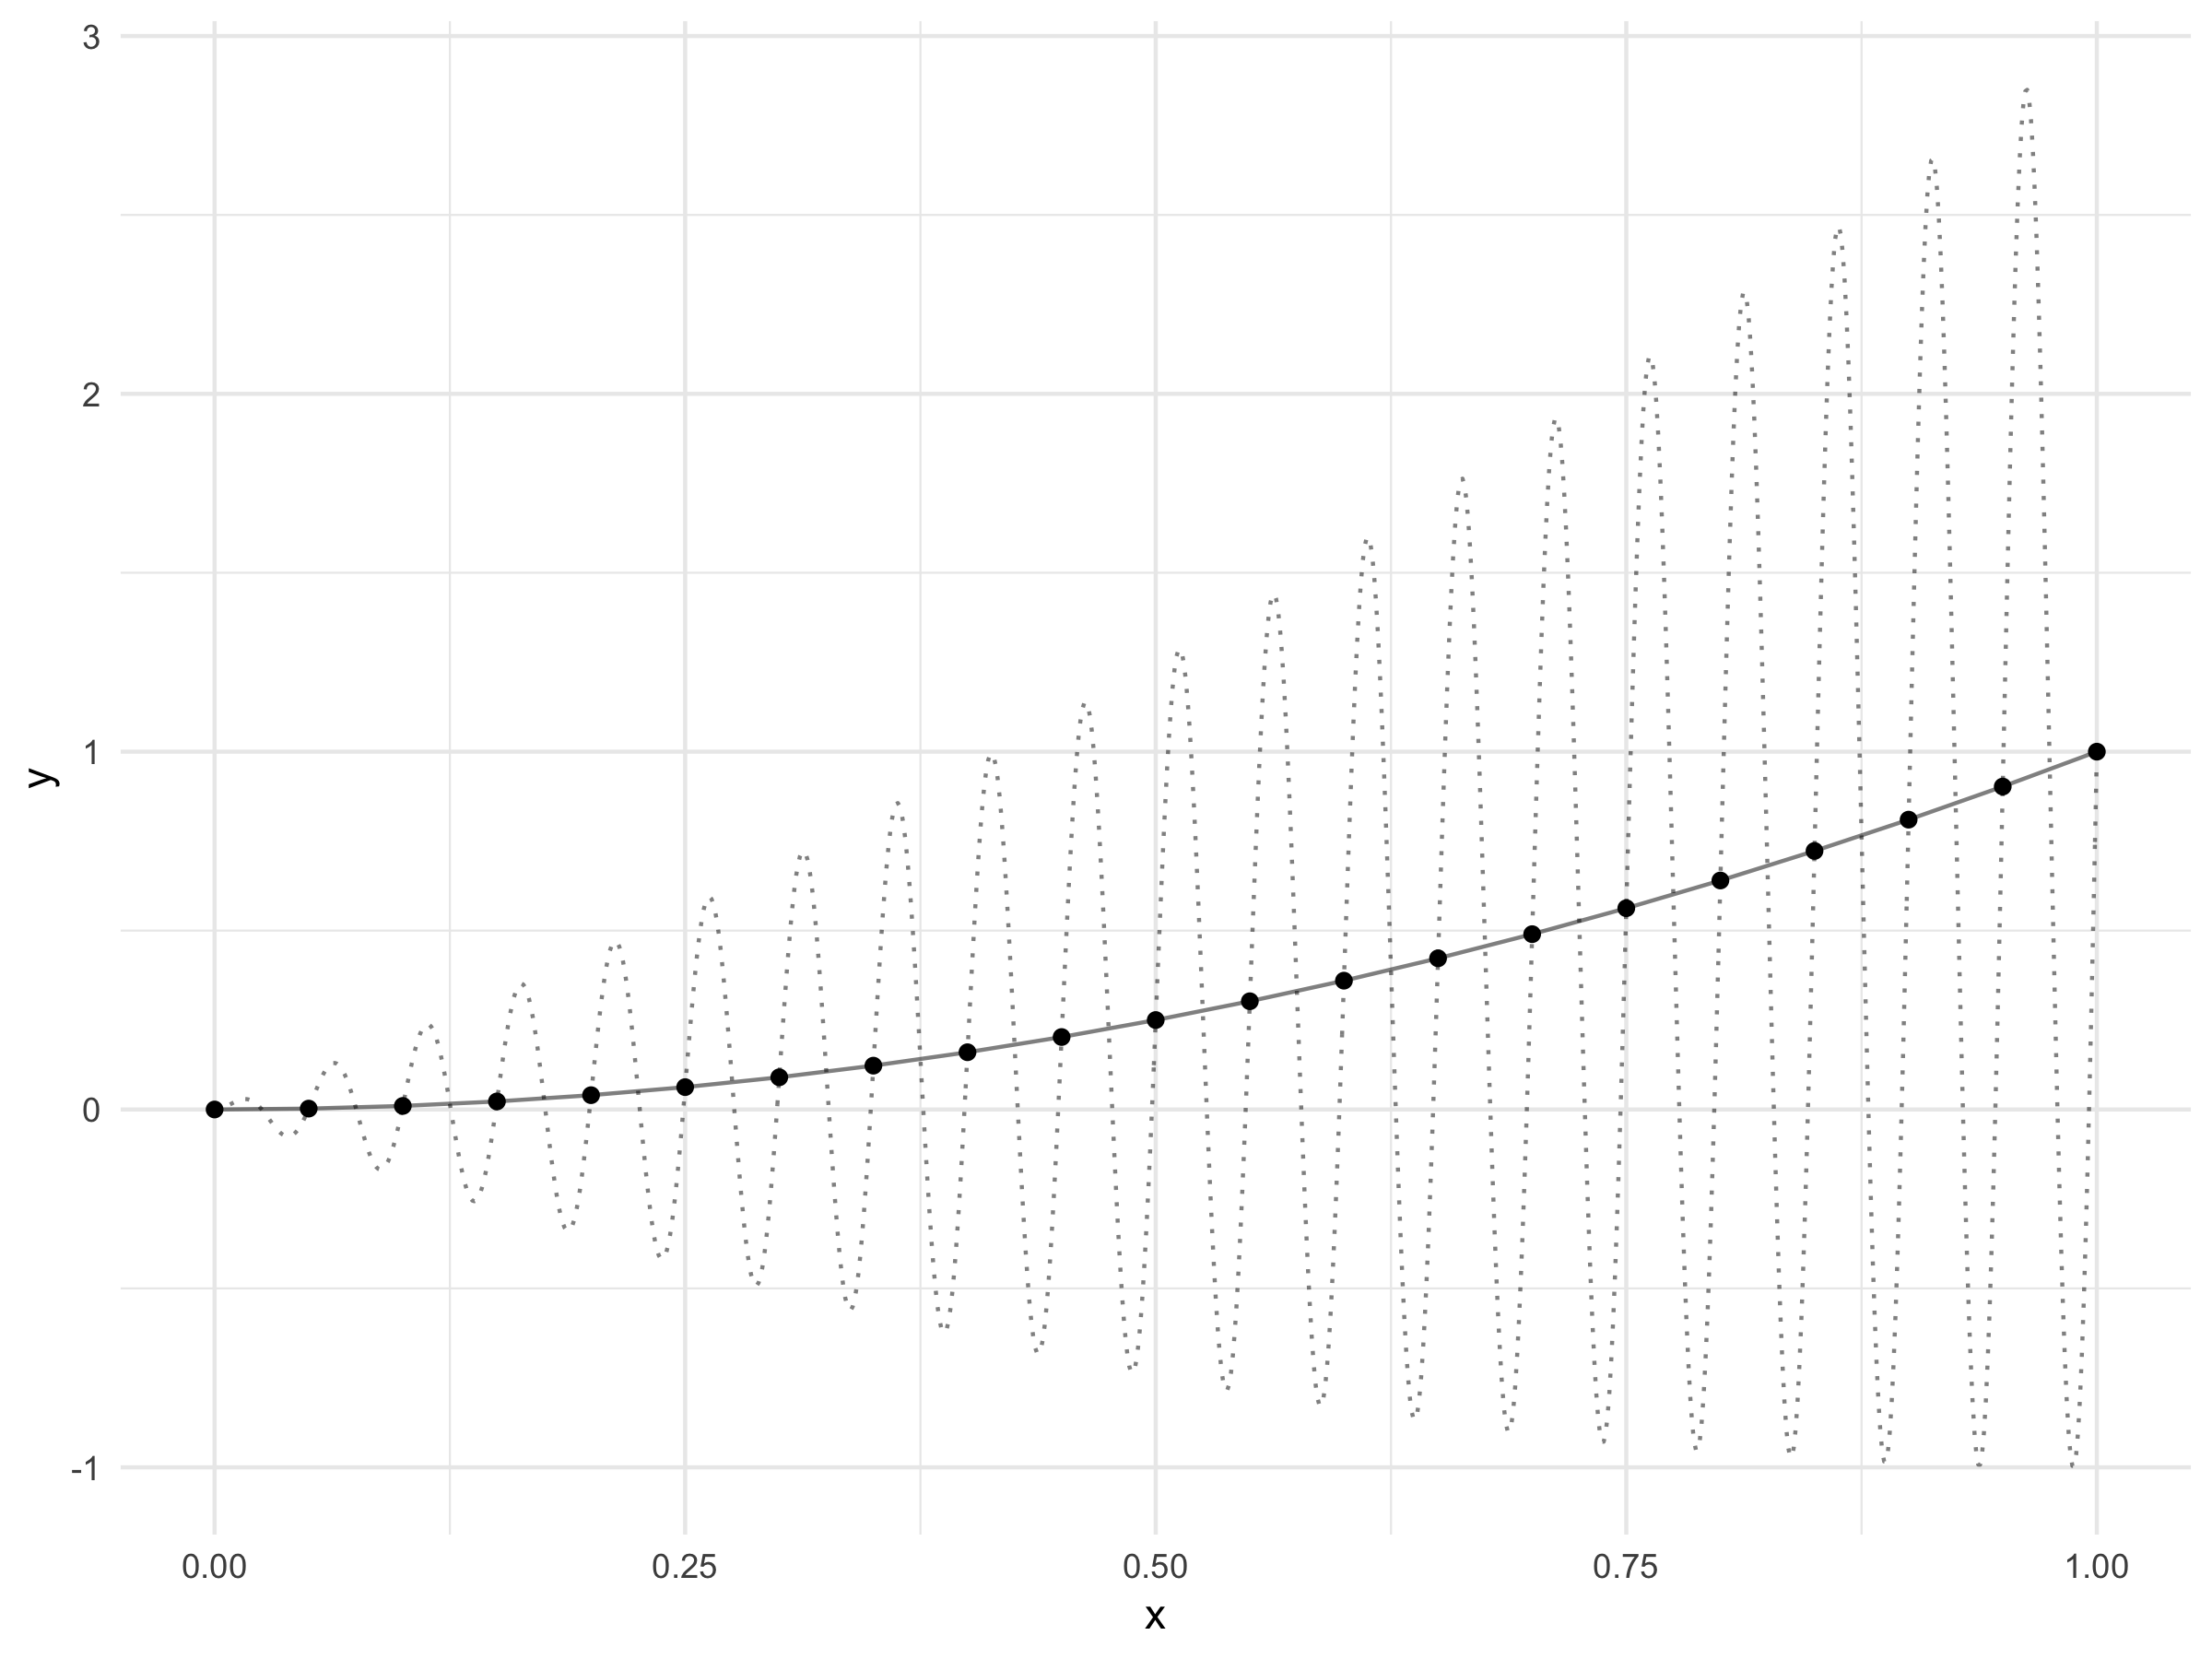
\includegraphics[width=\textwidth]{figures/sol01-fig02}
\end{center}

Notice that the predicted function $\widehat{f}$ perfectly fits the observed
training data, but would not do a very good job for new data observed at
different values of $x$ with the `true' function $f(x) = x^2$.

\vspace*{12pt}

\textbf{6. Consider the following small dataset:}

\begin{center}
\begin{tabular}{cc}
x & y \\ \hline
1 & 0 \\
2 & 1 \\
3 & 0 \\
4 & 0 \\
5 & 1 \\
6 & 1 \\
7 & 0 \\
8 & 1 \\
9 & 1 \\
10 & 1 \\
\end{tabular}
\end{center}

\textbf{Answer the following questions (you should be able to do this by hand):}

\textbf{What is the best split value derived from this data? What value does
your model predict will be the value of $y$ if $x = 1$? How about $x=10$ and
$x=5$?}

\vspace*{12pt}

The best split value is to use $x = 5$ as the cut-off, with messages containing
five or more capital letters being classified as spam. With this, we would
classify $x=1$ as `ham' and $x=10$ and $x=5$ as spam.

\vspace*{12pt}

\textbf{Using mis-classification loss, what is the loss of your model on this
dataset?}

\vspace*{12pt}

The mis-classification loss (or rate) is the proportion of training examples
that we missed. Here, we would \textit{falsely} classify the message with $2$
capital letters as spam and \textit{falsely} classify the message with $7$
capital letters as spam. All of the others are correct. This yields to a loss
of 20\%.

\vspace*{12pt}

\textbf{7. Take the following data as a \textit{test set} for the model you built
in the prior question:}

\begin{center}
\begin{tabular}{cc}
x & y \\ \hline
4 & 0 \\
4 & 1 \\
4 & 1 \\
8 & 0 \\
8 & 1 \\
8 & 0 \\
8 & 1 \\
\end{tabular}
\end{center}

\textbf{What is the misclassification rate on the test data? Is this value better or
worse than the loss function applied to the training data?}

\vspace*{12pt}

On this new data, we falsely classify one of the messages with $x=4$ as ham
and two of the $x=8$ messages as spam. This leads to a loss of 42.8\% ($\frac{3}{7}$),
not nearly as good as with the original data.

\vspace*{12pt}

\textbf{8. If you have not yet installed R, do that now. Using code similar to
that in the notes, redo the best split prediction using R. Does it give the
same output that you had when computing it by hand?}

\vspace*{12pt}

Here is the code to make this work (minus the function itself, which you can
find in the notes):

% casl_utils_best_split <-
% function(x, y)
% {
%   unique_values <- unique(x)
%   class_rate <- rep(0, length(unique_values))
%   for (i in seq_along(unique_values))
%   {
%     class_rate[i] <- sum(y == (x >= unique_values[i]))
%   }
%   unique_values[class_rate == max(class_rate)]
% }

\begin{rcode}
x <- c(1, 2, 3, 4, 5, 6, 7, 8, 9, 10)
y <- c(0, 1, 0, 0, 1, 1, 0, 1, 1, 1)

casl_utils_best_split(x, y)
\end{rcode}
\begin{rres}
[1] 5
\end{rres}

Exactly as we had by hand.

\vspace*{12pt}

\textbf{9. (optional) Modify the function \code{cnlp\_utils\_best\_split} so that
it also checks whether the best split would classify every value as a $1$ if
it is less than some cutoff value. Make sure that the output makes it clear
whether the cutoff is a less than or greater than value.}

\vspace*{12pt}

\begin{rcode}
casl_utils_best_split_improved <-
function(x, y)
{
  unique_values <- unique(x)
  class_rate_ge <- rep(0, length(unique_values))
  class_rate_le <- rep(0, length(unique_values))
  for (i in seq_along(unique_values))
  {
    class_rate_ge[i] <- sum(y == (x >= unique_values[i]))
    class_rate_le[i] <- sum(y == (x <= unique_values[i]))
  }
  if (max(class_rate_ge) >= max(class_rate_le))
  {
    print("Classify y=1 greater than or equal to cut-off(s)")
    class_rate <- class_rate_ge
  } else {
    print("Classify y=1 less than or equal to cut-off(s)")
    class_rate <- class_rate_le
  }
  unique_values[class_rate == max(class_rate)]
}
\end{rcode}

\vspace*{12pt}

\end{document}

